\section{Logical Addressing Schemes}
VM cost: Badly behaved program causes thrashing.

\subsection*{Segmentation for Address Translation}
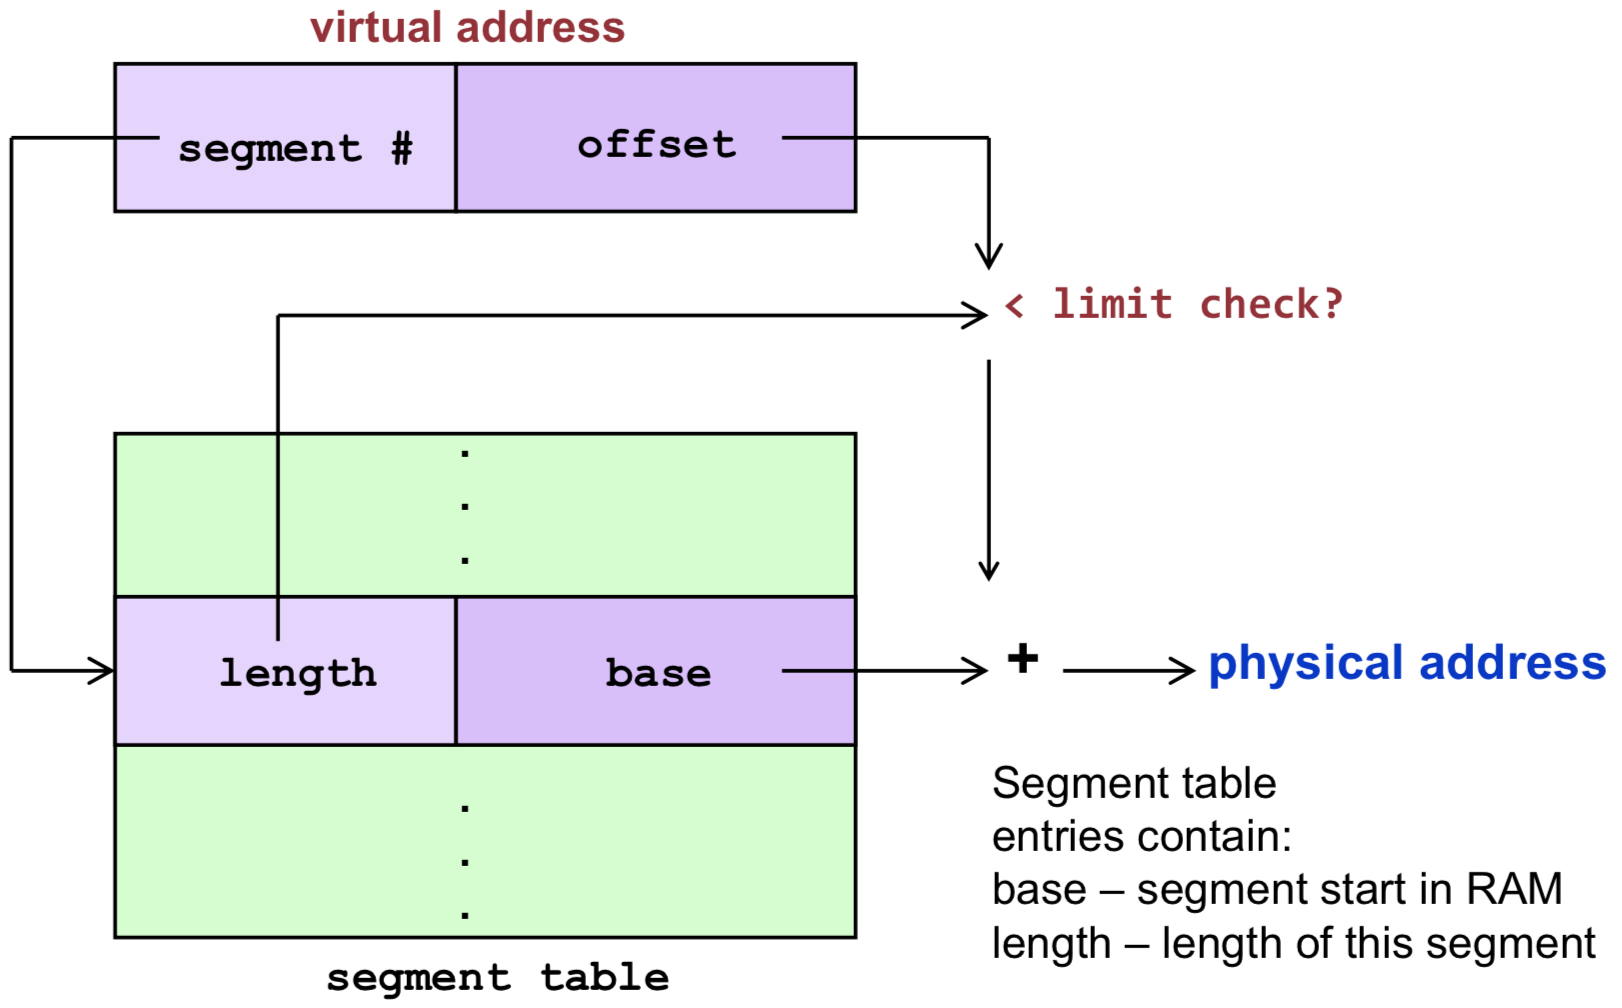
\includegraphics[width=0.75\linewidth]{images/segmentation-scheme}\\
permission info (read, write, exec -> invalid operation leads to seg fault).\\
(-)external fragmentation (but easier compaction), resizing causes framentation problems, may require explicitly selecting segments, swapping overhead high for large segments.

\subsection*{Paging for Address Translation}
Internal fragmentation, no external fragmentation. Rather than resizing, just use more pages. Overhead of page transfer to/from swap is on the order of few disk blocks.\\
\emph{Memory Sharing:} VM not needed for sharing, but allows logical address to be different and still share.\\
\emph{Direct Paging:}\\
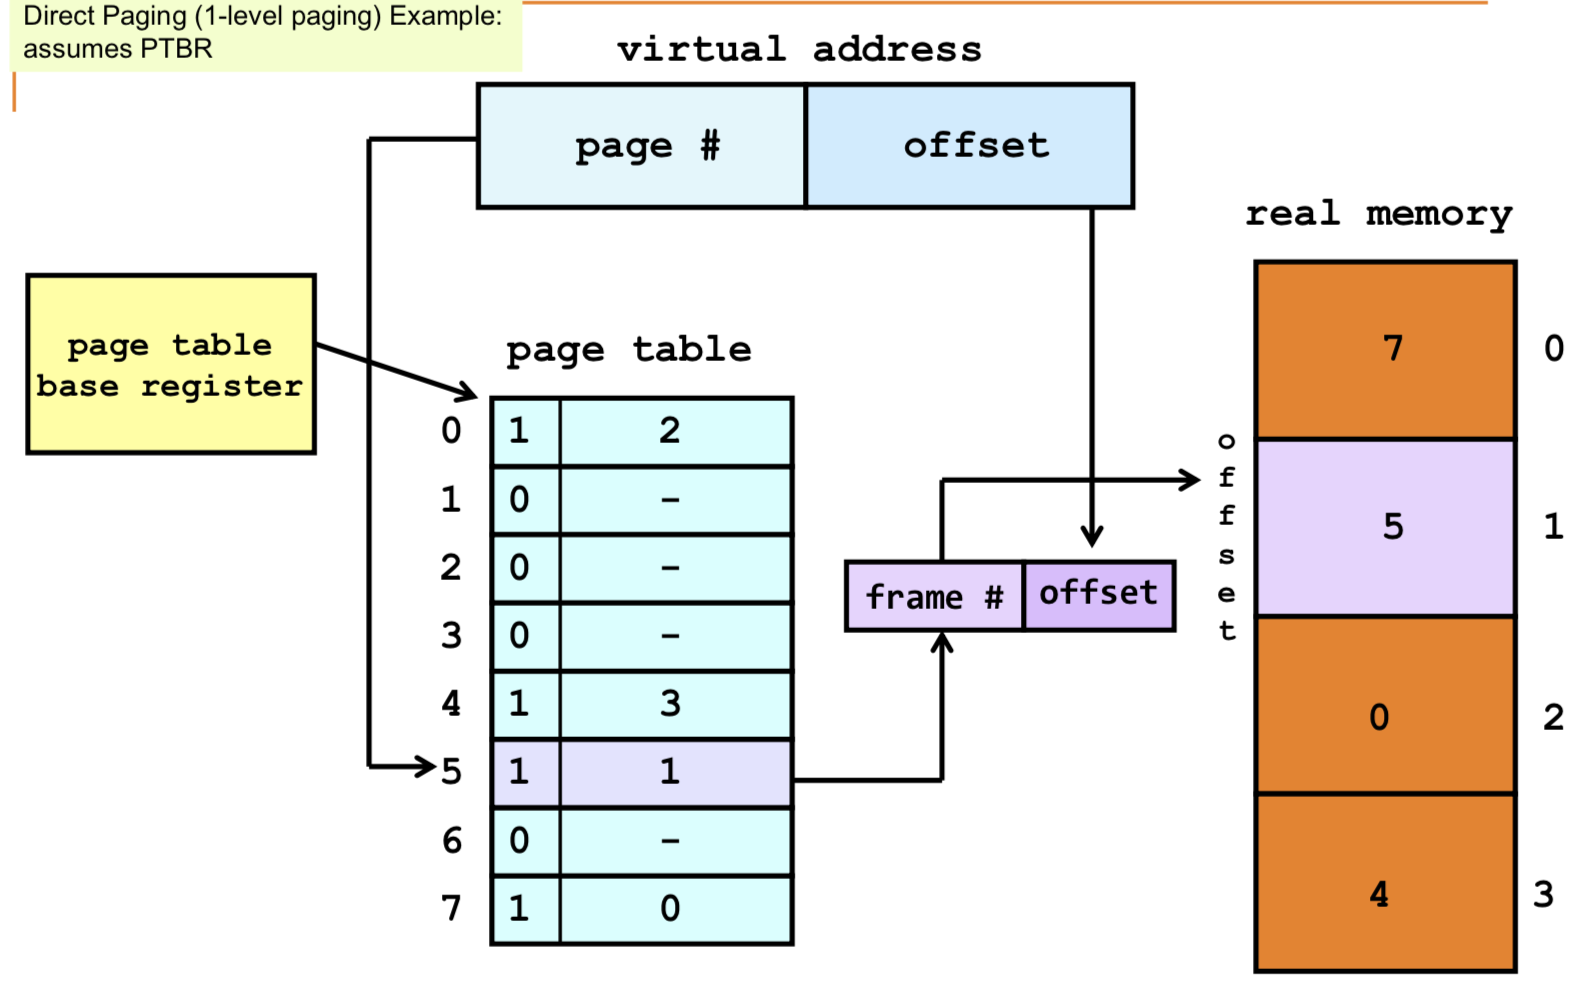
\includegraphics[width=0.8\linewidth]{images/direct-paging}\\
Overhead: page table size too big (same regardless of process memory usage)\\
\emph{2-level Paging:} save space\\
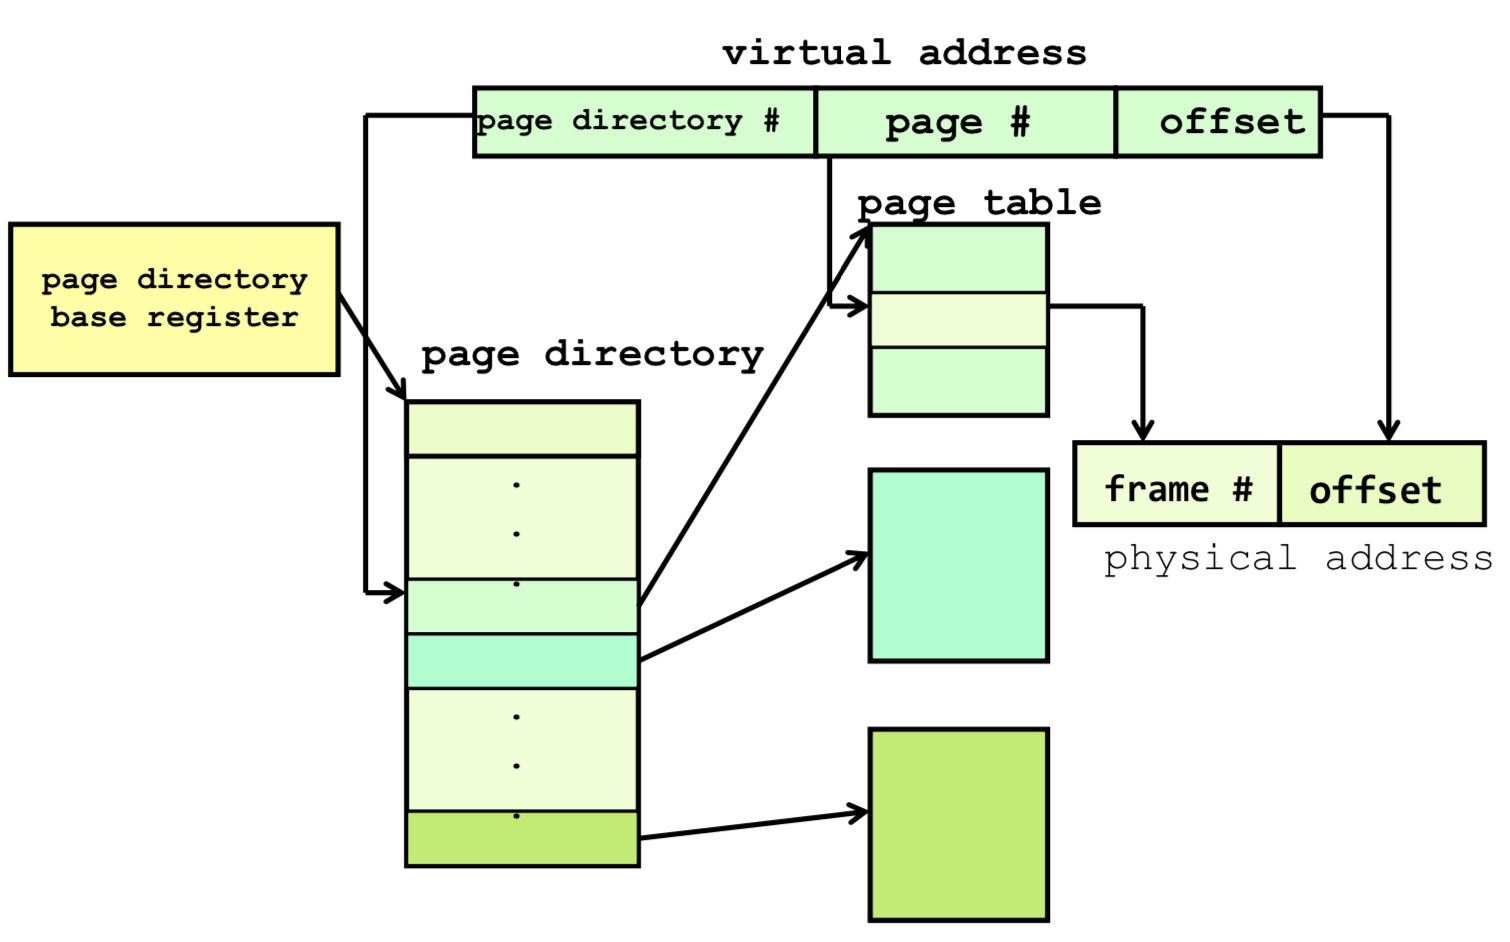
\includegraphics[width=0.8\linewidth]{images/2-level-paging}\\
\emph{Multi-level Paging:} tree with k levels for k-level paging, space savings when tree not complete. Pages tables can be in VM and be paged.\\
\emph{x86 hybrid paging: segmentation+paging:}\\
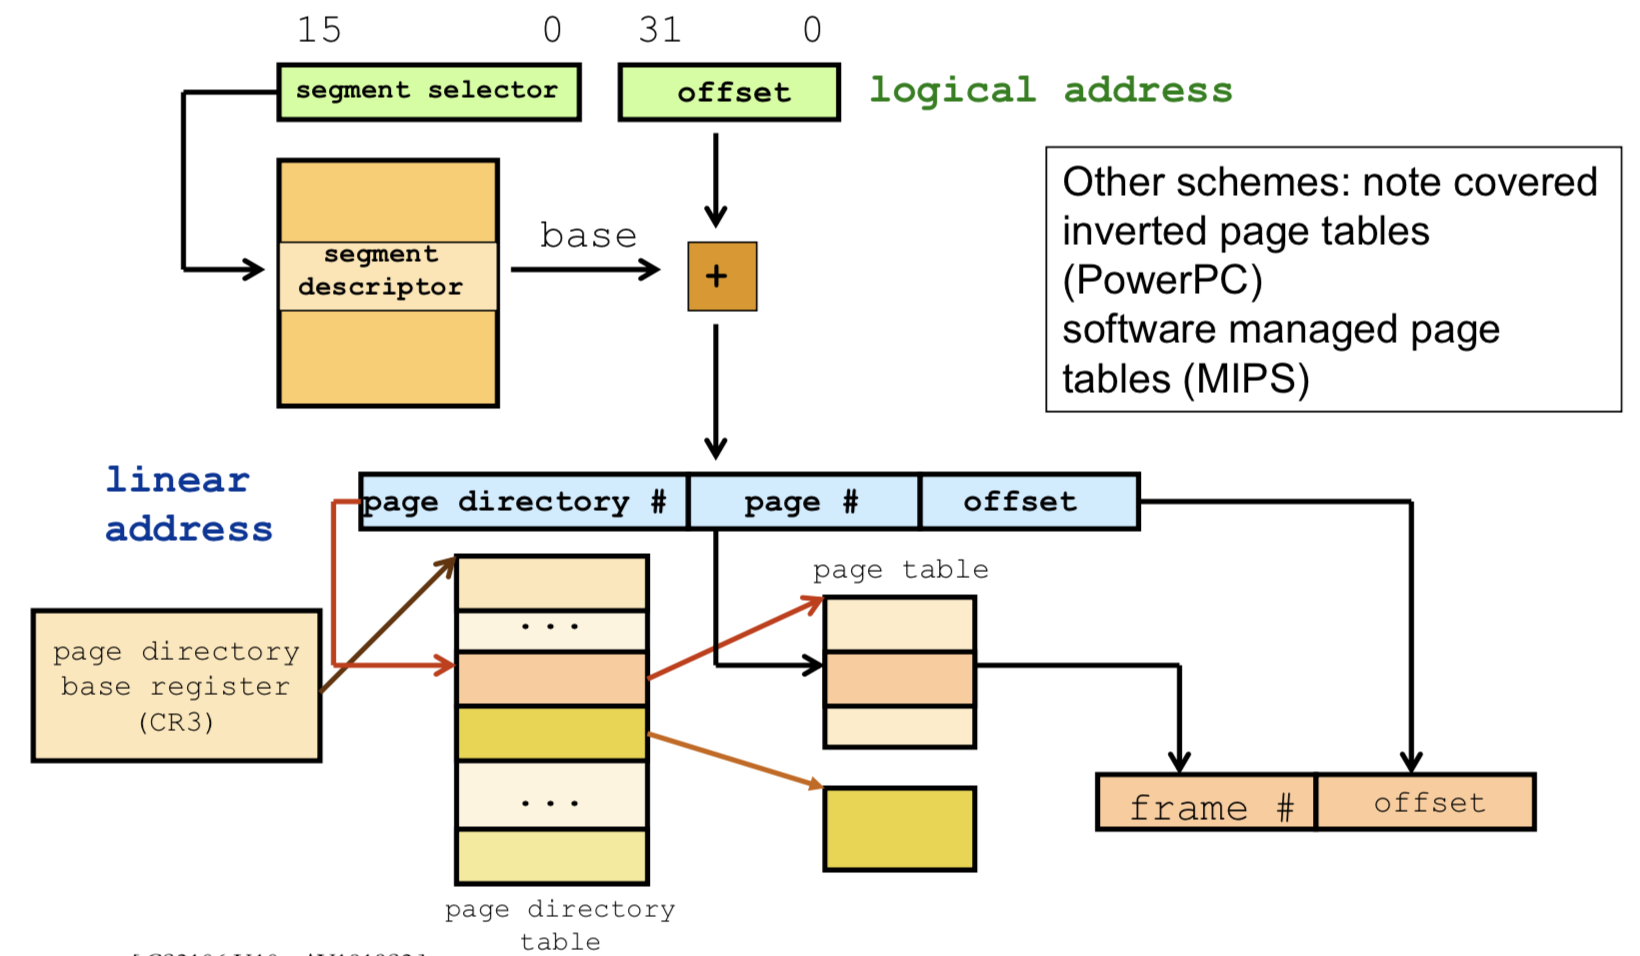
\includegraphics[width=0.8\linewidth]{images/x86-paging}

\subsection*{Page Table Entries (multi-level paging)}
\emph{Non-leaf nodes:} address of next level page table, valid bit. \emph{Leaf nodes:} frame, valid(present) bit - page present in RAM, dirty(modified) bit - set when page is written, referenced bit - set when page is used, protection bits - read/write/exec.

\subsection*{Translation Lookaside Buffer (TLB)}
$memory\_access\_time=m+(1-p) \ast 1+pkm) \approx m$ (k-level paging). Without cache: $(k+1)m$ (p=1). Context switch -> TLB flush, just invalidate entire TLB cache. x86: write to register CR3(PDBR) flushes TLB.